\section{基于$L_1$范数主成分分析的高维因子模型估计}

\subsection{因子分析简介}
因子分析是主成分分析的推广和发展,它也是多元统计中广泛使用的一种降维方法。
因子分析研究相关矩阵或者协方差矩阵的内部依赖关系,它将多个变量综合为少数几个因子,
以再现原始变量和因子之间的关系。

因子分析最早由英国心理学家Charles Spearman提出,最早用于智力测验得分数据的分析中。
现在因子分析在心理学、社会学、经济学等学科都取得了广泛应用。
\subsubsection{正交因子模型}

设$\bm{X} = (X_1, X_2, ..., X_p)^T$是可观测的随机向量,$\mathbb{E}\bm{X} = \bm{\mu}$,
$\mathbb{D}(\bm{X}) = \bm{\Sigma}$,设$\bm{f} = (f_1, f_2, ..., f_m)^T\\ (m <p)$为不可观测的随机向量,且
$\mathbb{E}\bm{f} = 0$,$\mathbb{D}(\bm{f}) = \bm{I}_m$(即$\bm{f}$的各分量方差为1,且互不相关)。最后,设
$\bm{e} = (e_1, e_2, ..., e_p)^T$和$\bm{f}$互不相关,并且
$$
    \mathbb{E}(\bm{e}) = \bm{0}\mbox{,}\mathbb{D}(\bm{e}) = diag({\sigma _1}^2, ..., {\sigma _p}^2)
    \mbox{为对角矩阵。}
$$
假设随机向量$\bm{X}$满足以下模型:
\begin{equation*}
\left\{
\begin{array}{clr}
    X_1 - \mu_1 = a_{11}f_1 + a_{12}f_2 + ... + a_{1m}f_m + e_1, \\
    X_2 - \mu_2 = a_{21}f_1 + a_{22}f_2 + ... + a_{2m}f_m + e_2, \\
    ... \\
    X_p - \mu_p = a_{p1}f_1 + a_{p2}f_2 + ... + a_{pm}f_m + e_p,
\end{array}
\right.
\end{equation*}
我们称该模型为正交因子模型,矩阵表示为:
$$
    \bm{X} = \bm{\mu} + \bm{A}\bm{f} + \bm{e}
    \eqno{(2-1)}
$$
其中$f_1, f_2, ..., f_m$称为$\bm{X}$的公共因子;$e_1, e_2, ..., e_p$称为$\bm{X}$
的特殊因子。公共因子一般对$\bm{X}$的每一个分量都起作用,而$e_i$一般仅仅对$X_i$起作用。
并且各个特殊因子之间以及特殊因子和所有公共因子之间都是不相关的。
其中$\bm{A} = (a_{ij})_{p \times m}$是待估计的系数矩阵,称为因子载荷矩阵。
$a_{ij}$称为第$i$个变量在第$j$个因子上的载荷,它反映了第$i$个变量在第$j$个因子上的相对重要性。

% 设$p$维随机向量$X=(X_1, X_2, ..., X_p)^T$的数学期望为$\mu = (\mu_1, \mu_2, ..., \mu_p)^T$,
% 协方差矩阵为$\Sigma$,假设$X$线性依赖于少数几个不可观测的随机变量$f_1, f_2, ..., f_m(m < p)$,和$p$个随机
% 误差项$e_1, e_2, ..., e_p$,一般称$f_1, f_2, ..., f_m$为公共因子,称$e_1, e_2, ..., e_p$为特殊因子或
% 误差,因子模型有如下表达式:
% $$ X = \mu + Af + e \label{a}  \eqno{(2-1)}$$
% 其中$f = (f_1, f_2, ..., f_p)^T$为因子,$A$是因子载荷矩阵,$e = (e_1, e_2, ..., e_p)^T$是特殊因子。
% 在式($2-1$)中,随机向量$X$围绕均值的波动由公共因子的线性组合加上一个特殊因子解释。
% 经典因子模型假设相互独立,$e_1, e_2, ..., e_p$相互独立并且$f$和$e$的样本之间相互独立。

\subsubsection{动态因子模型}

经典因子模型即正交因子模型提出后,迅速成为在心理学、社会学等多个学科内得到了广泛的使用。
然而因子模型在计量经济学研究领域的应用出现较晚,这可能是因为经典因子模型主要用于处理截面数据,
而计量经济学,尤其是宏观计量经济学的主要研究对象为时间序列数据。

Geweke与Sargent等人首先在计量经济学领域提出了动态因子模型,
动态因子模型是经典因子模型在时间序数据上的延伸,它提供了从维数众多的经济时间序列数据中提取公共因子来研究和解释
经济波动的手段。
动态因子模型的基本思想是:宏观经济具有周期性的波动是通过一系列经济变量的活动来传递和扩散的,
任何一个经济变量本身的波动都不足以代表宏观经济的整体波动。对于经济波动的研究需要从多个具有相依性的经济变量同时着手。
因此,需要从一国许多经济时间序列数据中估计出驱动各变量波动的共同动态因子,并且给出解释。
动态因子模型已经成为判别和分析经济周期波动的有效工具。

令$\bm{X}_t = (\bm{X}_{1t},\bm{X}_{2t}, ..., \bm{X}_{pt})^T$为一组宏观经济变量在$t$时刻的水平,并且$\bm{X}_t$可以表达为如下形式:
$$ \bm{X}_t = \lambda(L)\bm{f_t} + e_t \eqno{(2-2)}$$
其中,$\bm{f}_t$ 为$q\time 1$ 维的动态因子向量,$\lambda(L)$为由$s$阶滞后多项式算子组成的$p \times q$矩阵。
动态因子模型通常假设动态因子向量服从某一个向量随机过程。即动态因子模型
不仅允许观测变量受因子滞后项的影响,而且也允许因子本身具有独立的动态演化过程。

\subsubsection{近似因子模型}
在近似因子模型出现以前,DFM 主要应用于仅 包含几个总体宏观经济变量的小型数据集。这主要 是由于经济学家们假定影响所有变量的普遍性结构
冲击是经济变量协同变动的原因。然而在包含成百 上千个变量的大型经济数据集中,往往存在仅影响 某一组变量的部门冲击或局部冲击,
若根据经济理 论将这些非普遍性冲击归于异质性部分,则会造成 异质性部分截面相关,这又违背了经典因子模型中 异质性部分相互正交的假定。

因此,Chamberlain 和 Rothschild放弃 异质性部分的协方差矩阵为对角阵 的假定,允许异质性部分存在一定程度的截面相关, 
模型假设允许$f_t$的各个分量$f_1, f_2, ..., f_m$具有相依性,$e_1, e_2, ..., e_p$可以不独立,
并且允许$f_t$,$e_t$具有时间序列相依性。从而将模型扩展为了为动态近似因子模型。

% 通过放宽模型假设和形式变换,可以将动态因子模型转变为在经济变量预测中更加实用的静态近似因子模型。
% 令$X_t = (X_{1t},X_{2t}, ..., X_{pt})^T$为一组宏观经济变量在$t$时刻的水平,并且$X_t$可以表达为如下形式:
% 其中$f_t$是$q$维的动态相依因子向量,$\lambda(L)$为由$s$阶滞后多项式算子组成的$p \times q$矩阵。近似因子
% 模型的模型假设允许$f_t$的各个分量$f_1, f_2, ..., f_m$具有相依性,$e_1, e_2, ..., e_p$可以不独立,


% 令某一个经济指标$y$在$t+h$时刻的水平为$y_{t+h}$,则其预测值由式($2-4$)给出:
%     $$X_t = AF_t + e_t $$
%     $$y_{t+h} = \beta F_t + \beta _yy_t + \varepsilon _{t+h} \eqno{(2-4)}$$
% 其中$\beta F_t$包括了近似因子$t$时刻的当期项和滞后项,$\beta _yy_t$代表了指标$y$受自身滞后项的影响,$\varepsilon _{t+h}$
% 为预测误差。

\subsection{因子模型的估计}
% 在$2.1$节中提出,使用因子模型进行分析的关键是找出最具贡献的因子,而关键步骤就是要估计因子载荷矩阵。
% 对于($2-1$)中的因子模型,假设我们已知$p$个相关变量的观测值
% $$\bm{X}_{(i)} = (x_{i1}, ..., x{i_p})^T (i = 1, 2, ..., n)$$
对于正交因子模型,
在因子载荷矩阵$\bm{A}$中,我们计算各列的平方和,记为$q_j^2$,即
$$
    q_j^2 = \sum_{i=1}^p a_{ij}^2 (j = 1, 2, ..., m)
$$
$q_j^2$表示第$j$个公共因子$f_j$对$\bm{X}$的所有分量的总影响,称为公共因子$f_j$对$\bm{X}$的
方差贡献。因此如果我们列出$\bm{A}$的所有列平方和,按照方差贡献大小就可以选出最有影响的公共因子。
因此因子分析的关键步骤就是估计出因子载荷矩阵。

对于正交因子模型可以通过主成分法、主因子法和极大似然法来估计因子载荷矩阵。不可观测的公共因子有时候也需要进行估计,
例如用来诊断因子模型或者作为进一步分析的原始数据,这就需要我们给出因子得分,一般在得出了因子载荷矩阵之后,
对于因子得分,可以通过加权最小二乘法(巴特莱因子得分)或者通过回归法(汤普森因子得分)进行估计。

但是对于动态因子模型和近似动态因子模型,因为不满足正交因子模型的一些关键模型假设,因此需要不同的估计手段。

\subsubsection{动态因子模型的估计}
动态因子模型的提出者Geweke和Sargent等人都是使用频域方法估计模型,这种方法不能够直接估计出动态因子$\bm{f}_t$,
因此也就不能将因子作为预测或者扩展模型等用途。使得动态因子模型的应用收到限制。
由于动态近似因子模型估计困难,因此在预测中,往往使用模型的静态形式:
$$X_t = AF_t + e_t \eqno{(2-3)}$$
式($2-3$)中,$F_t$是$m$维向量,称为静态因子,即$F_t$仅在当期影响$X_t$(因为$F_t$包括了动态因子$f_t$的当期项和
滞后项),它本身可以不具有经济学含义。$A$是因子载荷矩阵。本文采用式($2-3$)中的模型进行宏观经济指标的预测。

对于静态形式的估计,Stock和Watson于1989年最早提出了一种方法:这种方法采用
Kalman 滤波构造似然 函数,并采用极大似然方法来估计参数。
这种方法的 优点是: 在误差项服从正态分布的假定下,能够得到 因子的有效估计量。
然而,由于在估计参数过程中 会应用到非线性数值优化算法,而待估参数的个数与变量维数$p$成比例,
限于当时的计算能力,这种方法只能用于处理低维的精确动态因子模型。

针对维数很高的宏观经济变量,Stock和Watson于2002年给出了一种非参数的方法,并且得到广泛使用。
这种方法使用主成分分析法进行估计,对式($2-3$),因子载荷矩阵$\bm{A}$的估计量$\hat{\bm{A}}$即为
$\bm{X}_t$的样本协方差矩阵$$\hat{\bm{\Sigma}}_{\bm{X}} = \frac1{n}\sum_{t=1}^n\bm{X_t}\bm{X_t}^T
\eqno{(2-4)}$$的前
$r$个最大特征值所对应的特征向量组成的$p\times r$维矩阵,因子的主成分估计量为:
$$ \hat{\bm{F}}_t = \frac1{p}\hat{\bm{A}}\bm{X}_t 
\eqno{(2-5)}$$

主成分估计量具有一系列良好的性质。例如, 在$p \rightarrow \infty$, $n \rightarrow \infty$ 且 $p^2 / n \rightarrow \infty$
的条件下,主成分估计量$\hat{\bm{F}}_t$是因子空间的一致估计量,且在随后的建模 过程中可以当作观测到的数据。

\subsubsection{主成分分析法}
主成分分析法(principal component analaysis, PCA)已经是十分常见的数据降维方法,这里我们不对主成分分析法做详细介绍,仅针对我们的问题,
下面给出使用主成分分分析法计算出估计量的步骤:

记矩阵$\bm{X}_{p\times n}$为$p$维宏观经济变量$\bm{X}_t$在$t_1, ..., t_n$的$n$次观测,

1. 将$\bm{X}$进行中心化;

2. 计算样本协方差矩阵$\frac1{n}\bm{X}\bm{X}^T_{p\times p}$;

3. 对样本协方差矩阵特征值分解,并从小到大排列这些特征值;

4. 因子载荷矩阵估计量$\hat{\bm{A}}_{p\times m} (m < p)$为前$r$个特征值对应的特征向量组成的矩阵。

不难看出,主成分分析法进行估计的关键计算步骤是对样本协方差矩阵的特征值分解。

\subsubsection{奇异值分解} 
这里有必要简要介绍奇异值分解(singular value decomposition, SVD),它也是一类常用的降维方法,在常用统计软件包中
PCA问题的计算往往转化成奇异值分解问题求解。

奇异值分解解决将矩阵$\bm{A}$分解成正交矩阵$\bm{U}$和对角矩阵$\bm{\Sigma}$和另一正交矩阵$\bm{V}^T$的问题,即
$$
    \bm{A}_{m \times n} = \bm{U}_{m \times m}\bm{\Sigma}_{m \times n}\bm{V}_{n \times n}^T
$$

奇异值分解求解的关键就是得到奇异值,而后者是$\bm{A}^T\bm{A}$的特征值的平方根,即奇异值分解的关键计算步骤是对
$\bm{A}^T\bm{A}$进行特征值分解。这里假设我们取$\bm{A} = {\bm{X}^T}/{\sqrt{m}}$,不难看出和PCA问题等价。
因此所有的PCA问题可以转化为SVD进行求解,这样做的原因是高维矩阵进行特征值分解的效率很低,而SVD问题有不需要进行
特征值分解的更高效的迭代计算方法。


\subsection{$L_1$范数主成分分析}

Stock和Watson提出的主成分估计量等价于通过下面的$L_2$范数优化问题来估计$\bm{A}$和$\bm{F}$,即

$$
\hat{A}_{p\times m}, \hat{F}_{m\times n} = \underset{A,F}{\operatorname{arg\ min} } \|X - A\bm{F}\|_{L_2}
 = \underset{A, \bm{F}}{\operatorname{arg\ min}} \sum_{i=1}^p \sum_{j=1}^m (x_{ij} - a_i^Tf_i)^2 
\eqno{(2-6)}
$$

上述问题不是一个凸优化问题,我们可以转化为等价的PCA问题或者SVD问题解决。但是我们采用的等价解决方法具有
所有的$L_2$范数优化方法普遍的缺陷,那就是对离群值十分敏感。并且PCA和SVD方法都不能够直接处理具有缺失值的数据,
因此对于缺失数据必须进行插补。

然而由于各种原因,高维宏观经济数据中往往具有大量的缺失值和离群值,这就给因子模型的估计带来很多的麻烦,
从而进一步使用因子的估计量进行预测可能会变得不够准确。


\subsubsection{使用$L_1$范数}
将式($2-6$)中的目标函数更换为使用$L_1$范数,可得
$$\hat{\bm{A}}_{p\times m}, \hat{\bm{F}}_{m\times n} = \underset{\bm{A},\bm{F}}{\operatorname{arg\ min} } \|X - \bm{A}\bm{F}\|_{L_1}
= \underset{\bm{A}, \bm{F}}{\operatorname{arg\ min}} \sum_{i=1}^p \sum_{j=1}^m |x_{ij} - a_i^Tf_i| \eqno{(2-7)}$$
其中$\|.\|_{L_1}$表示矩阵的$L_1$范数。

式($2-7$)中定义的问题不是一个凸优化问题。但是一旦矩阵$\bm{A}$或者$\bm{F}$固定为常数,那么该问题就成为了一个凸优化问题,
可以找到全局最优解。这启发我们可以使用交替优化的方法求解这个优化问题,即每一步固定$\bm{A}$或者$\bm{F}$的值,来求解另一个
参数。

$$
F^{(t)} = \underset{F}{\operatorname{arg\ min}} \|X - \bm{A}^{(t-1)}\bm{F} \|_{L_1} \eqno{(2-8a)}
$$
$$
\bm{A}^{(t)} = \underset{\bm{A}}{\operatorname{arg\ min}} \|X - \bm{A}F^{T(t)}\|_{L_1} \eqno{(2-8b)}
$$

我们改写式($2-8a$)中的目标函数,
$$
E(F) = \|X - \bm{A}^{(t-1)}\bm{F} \|_{L_1} = \sum_{j=1}^{n}|x_j - \bm{A}^{(t-1)}f_j| \eqno{(2-9)}
$$
其中$x_j$是矩阵$X$的第j列,$f_j$是$\bm{F}$的第j列。于是式($2-8a$)中的问题可以分解为$n$个独立的子优化问题,
求解相应的$f_j$:
$$
    f_j = \underset{\theta}{\operatorname{arg\ min}} |\bm{A}^{(t-1)}\theta - x_j|
    \eqno{(2-10)}
$$

\subsubsection{缺失值处理}
在使用PCA和SVD时我们需要对矩阵$X$进行缺失值插补,然后才能进行计算。
在$L_1$算法中我们不需要进行缺失值插补,在式($2-11$)中,遇到$x_j$具有缺失值的场合,我们直接舍弃相应的
约束条件即可。
我们改写式($2-9$),
$$E(F) = \sum_{i=1}^d \sum_{j=1}^n |x_{ij} - a_i^Tf_j|$$
如果某个项$x_{ij}$缺失,我们直接舍弃目标函数中的对应累加项,在上述算法中对应的做法就是直接删除($2-11$)中的一个约束条件。

\subsubsection{算法步骤}
我们已经发现可以通过交替优化的方法求解式($2-7$)中的优化问题,下面我们更加详细地讨论$L_1$因子分析算法一些细节和具体实现步骤。

(一)初始化

和其他所有的迭代算法一样,在算法开始时,首先我们需要给$\bm{A}$一个初始值$\bm{A}^{(0)}$。对于$\bm{A}$可以采用简单随机数进行初始化,这里我们
为了加快收敛速度,可以使用经过缺失值插补(这里我们使用均值插补)后通过PCA算法进行得到的因子载荷矩阵作为$\bm{A}^{(0)}$。
在本章后续小结的实验中我们可以发现,在含有大量缺失值和离群值的条件下,两种不同的初始化方法最终结果差异并不大。

(二)收敛性

因为目标函数$E(\bm{A}, F) = \|X - \bm{A}\bm{F}\|_{L_1}$在每一个交替的优化步骤中都递减,并且$E(\bm{A},F)$具有下界($\geq 0$)。
因此交替优化算法一定收敛。因此我们可以设定一个收敛域值来停止迭代,这里我们设置终止条件:
    $$ \theta(a_i^{(t)}, a_i^{(t-1)}) <  \alpha $$
这里$\theta(a, b)$表示向量$a$和$b$的夹角;其中$a_i$是$\bm{A}$或者$F$的第i列;$\alpha$是一个很小的正数。

(三)算法步骤

下面我们给出$L_1$因子分析算法的计算步骤:

1.初始化:给出$\bm{A}$,$\Sigma$的初始值$\bm{A}^{(0)}$,$\Sigma^{(0)} = I$,(其中$\Sigma$为一对角矩阵,
$I$为单位矩阵);

2.交替凸优化:对于迭代次数$t = 1, ..., $收敛:
$$F^{(t)} = \underset{F}{\operatorname{arg\ min}} \|X - \bm{A}^{(t-1)}\Sigma^{(t-1)}F^{T}\|_{L_1}$$
$$\bm{A}^{(t)} = \underset{\bm{A}}{\operatorname{arg\ min}} \|X - \bm{A}\Sigma^{(t-1)}F^{T(t)} \|_{L_1}$$
\begin{equation*}
    \text{归一化:}\left\{
                 \begin{array}{clr}
                 N_a = diag(\bm{A}^{(t)T}\bm{A}^{(t)})\\
                 N_f = diag(F^{(t)T}F^{(t)})\\
                 F^{(t)} \leftarrow F^{(t)}N_f^{-1}\\
                 \bm{A}^{(t)}\leftarrow \bm{A}^{(t)}N_a^{-1}\\
                 \Sigma^{(t)} \leftarrow N_a\Sigma^{(t-1)}N_f\\
                 \end{array}
    \right.
\end{equation*}

3.输出结果:$F \leftarrow F\Sigma^{1/2}$,$\bm{A} \leftarrow \bm{A}\Sigma^{1/2}$

\subsection{稳健性实验}
为了检验$L_1$因子分析算法在处理含有大量离群值和缺失值的数据时的稳健性,我们进行模拟实验,来对比采用$L_1$因子分析算法
和PCA因子分析,SVD因子分析以及采用$L_2$目标函数这几种方法的效果。

\subsubsection{数据准备}
为了进行模拟实验,我们首先需要随机产生一个高维低秩的矩阵来模拟高维宏观经济数据集。
我们产生一个$n$维方阵$M$,其中每一个随机元素均服从$[-100, 100]$的均分分布。然后我们对方阵$M$进行奇异值分解
,$M = U\Sigma V^{T}$。假设我们需要产生的低秩矩阵的秩为$r$,则$$X = U_{(:,1:r)}\Sigma_{(1:r,1:r)}V^T_{(:,1:r)}$$
即为我们得到的模拟高维低秩矩阵。

之后我们可以设置一定比例的缺失值和离群值,首先我们在矩阵的左下角剔除部分元素。在剩下的元素中,我们随机选取一部分
然后重新产生随机元素,每个元素服从$[-2000,2000]$上的均匀分布。图2.1展示了一个$30\times30$秩为3的
矩阵在模拟了缺失值和离群值后的情况。

\begin{figure}[H]
    \centering
    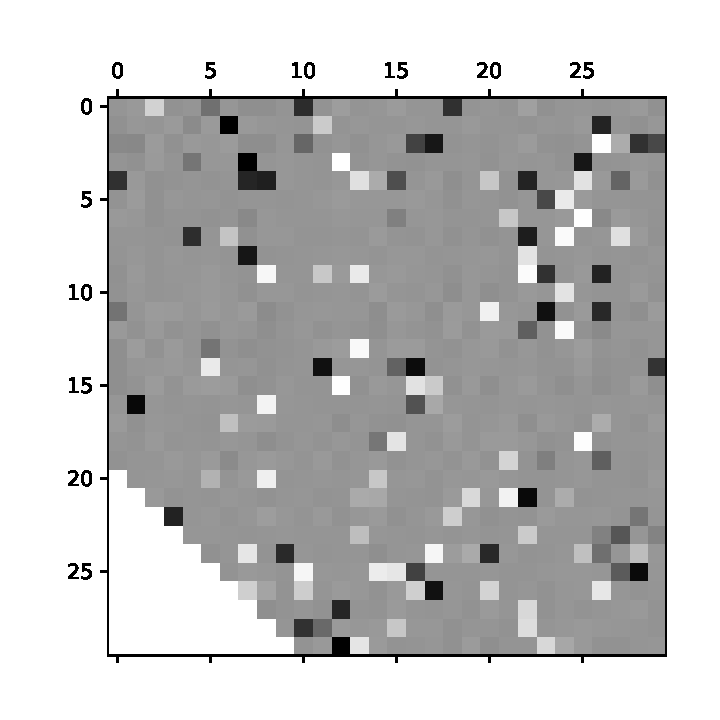
\includegraphics[width=.5\textwidth]{pics/matrix.pdf}
    \caption{\small $30\times30$的模拟矩阵,左下角白色代表缺失值,图中灰度越深代表元素的绝对值越大,因此深黑色的点代表了离群值}
    \label{fig2.1}
\end{figure}

\subsubsection{实验结果}
基于获得的高维低秩矩阵,我们主要比较四种获得因子估计量的方法:1)PCA,需要进行缺失值插补,这里我们使用均值插补法;2)SVD
,同样使用均值插补;3)基于$L_1$范数的估计方法,可以直接处理原始数据;4)一种基于加权$L_2$范数的估计方法(Black和Rangarajan,1996),
通过将($2-6$)损失函数加上随迭代变化的权重,可以直接处理原始数据。

令$\hat{\bm{X}} = \hat{\bm{A}}_{N \times M}\hat{\bm{F}}_{M \times N}$,我们比较因子残差
$\bm{E} = \hat{\bm{X}} -\bm{X}$。观察因子残差的平方的分布情况,
试验每一种算法作用在无干扰数据上和干扰后数据上的情况。

对于无干扰数据,每一种算法都具有很好的表现;
对于进行了缺失值和离群值模拟的数据,我们每组试验(给定$M$,$ N$)下均重复多次取平均值,图2.3给出了一个典型结果。
\begin{figure}[H]
    \centering
    \begin{minipage}[t]{0.48\textwidth}
    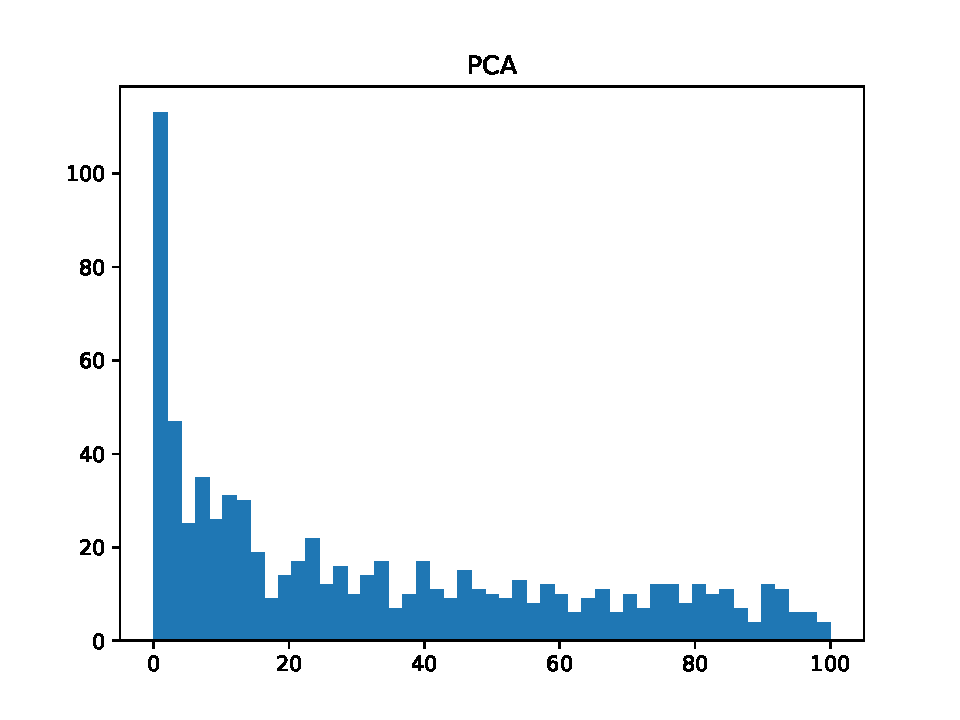
\includegraphics[width=8cm]{pics/lab1/pca-ab.pdf}
    \end{minipage}
    \begin{minipage}[t]{0.48\textwidth}
    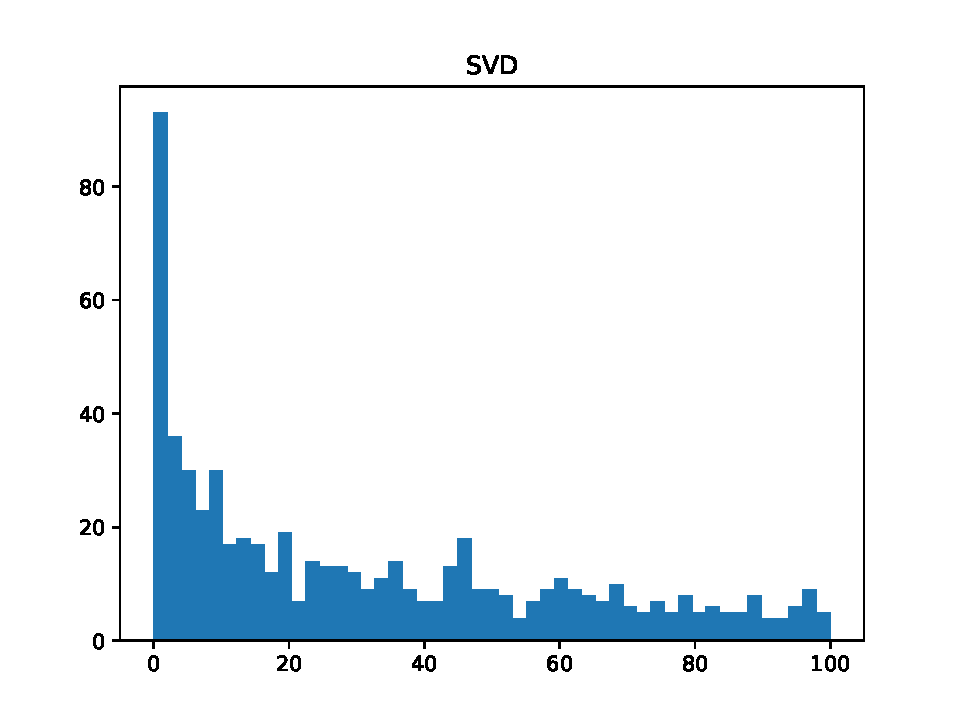
\includegraphics[width=8cm]{pics/lab1/svd-ab.pdf}
    \end{minipage}
    \begin{minipage}[t]{0.48\textwidth}
    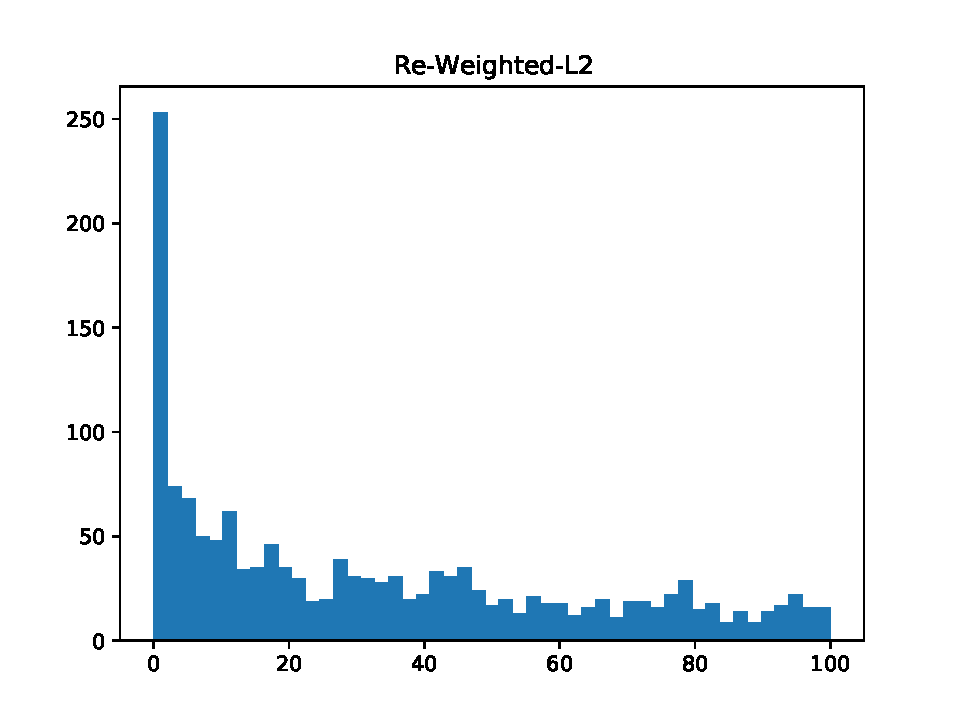
\includegraphics[width=8cm]{pics/lab1/l2-ab.pdf}
    \end{minipage}
    \begin{minipage}[t]{0.48\textwidth}
    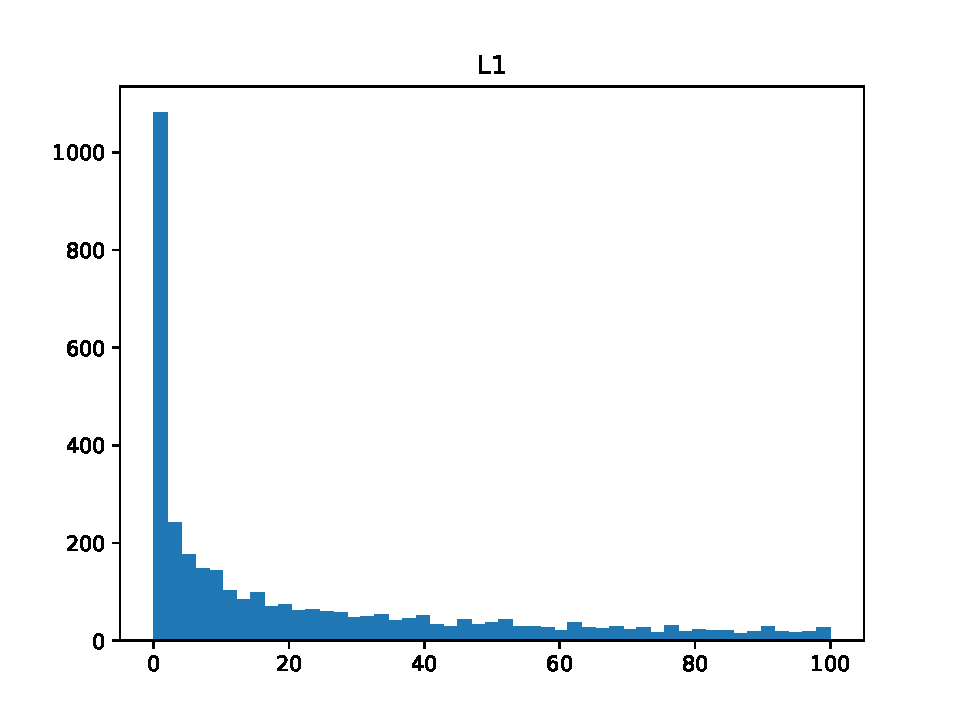
\includegraphics[width=8cm]{pics/lab1/l1-ab.pdf}
    \end{minipage}
    \caption{\small 图示为取$N = 80, M=3$,缺失值和离群值比例均为$10\%$的情况下,多次实验中平均因子残差的平方的分布情况。
    可以看出采用基于$L_1$范数进行估计,因子残差表现最好。}
\end{figure}

\subsubsection{结论}
实验表明,$L_1$范数主成分分析相比$L_2$主成分分析法和其他基于$L_2$范数优化的方法相比具有更好的稳健性,
特别适合于处理具有大量离群值的数据。

\subsection{基于国内主要月度宏观经济数据的实证研究}

\subsubsection{数据说明}
我们搜集了来自中国国家统计局、中国人民银行、海关总署、中国人力资源市场监测中心等部门以及国泰安经
济研究数据库从1999年9月至2019年6月主要公开月度(部分季度)宏观经济指标。
其中我们人为筛选出涵盖了宏观经济中实际产出(工业增加值增长率、能源产量增长率等)、
价格指数(如CPI、PPI、房地产价格指数等)、进出口(进、出口同比增速等)、
财政(公共财政收入、支出等)、金融(包括货币、信贷增速以及股票市场成交额和证券发行量等)、
各种景气指数(包括消费者信心指数、消费者预期指数、制造业采购经理指数等)、
消费和零售(各类消费品零售总额增速、居民收入变化率等)、
投资(包括固定资产投资增长、房地产投资增长、外商投资等)共计117个指标的月度时间序列。

对不平稳的增长率数据,我们对其进行一阶差分(存在季节效应的进行季节差分),对于非增长率数据,
我们对其进行对数一阶差分(存在季节效应的数据进行对数季节差分),仍然不能平稳的数据再次进行二阶差分。
之后所有数据均进行标准化处理。我们没有剔除任何离群值。

由于某些指标曾多次改变统计口径、统计频率等原因,这些数据中包含许多的缺失数据。
另外,在1999~2019年这20年间,中国经济经历了许多次重大外部冲击,许多经济指标中含有大量离群值(见图3),
从各指标的经验分布的峰度值来看,经济指标的分布存在尖峰厚尾现象。
\begin{figure}[H]
    \begin{minipage}[t]{1\textwidth}
    \centering
    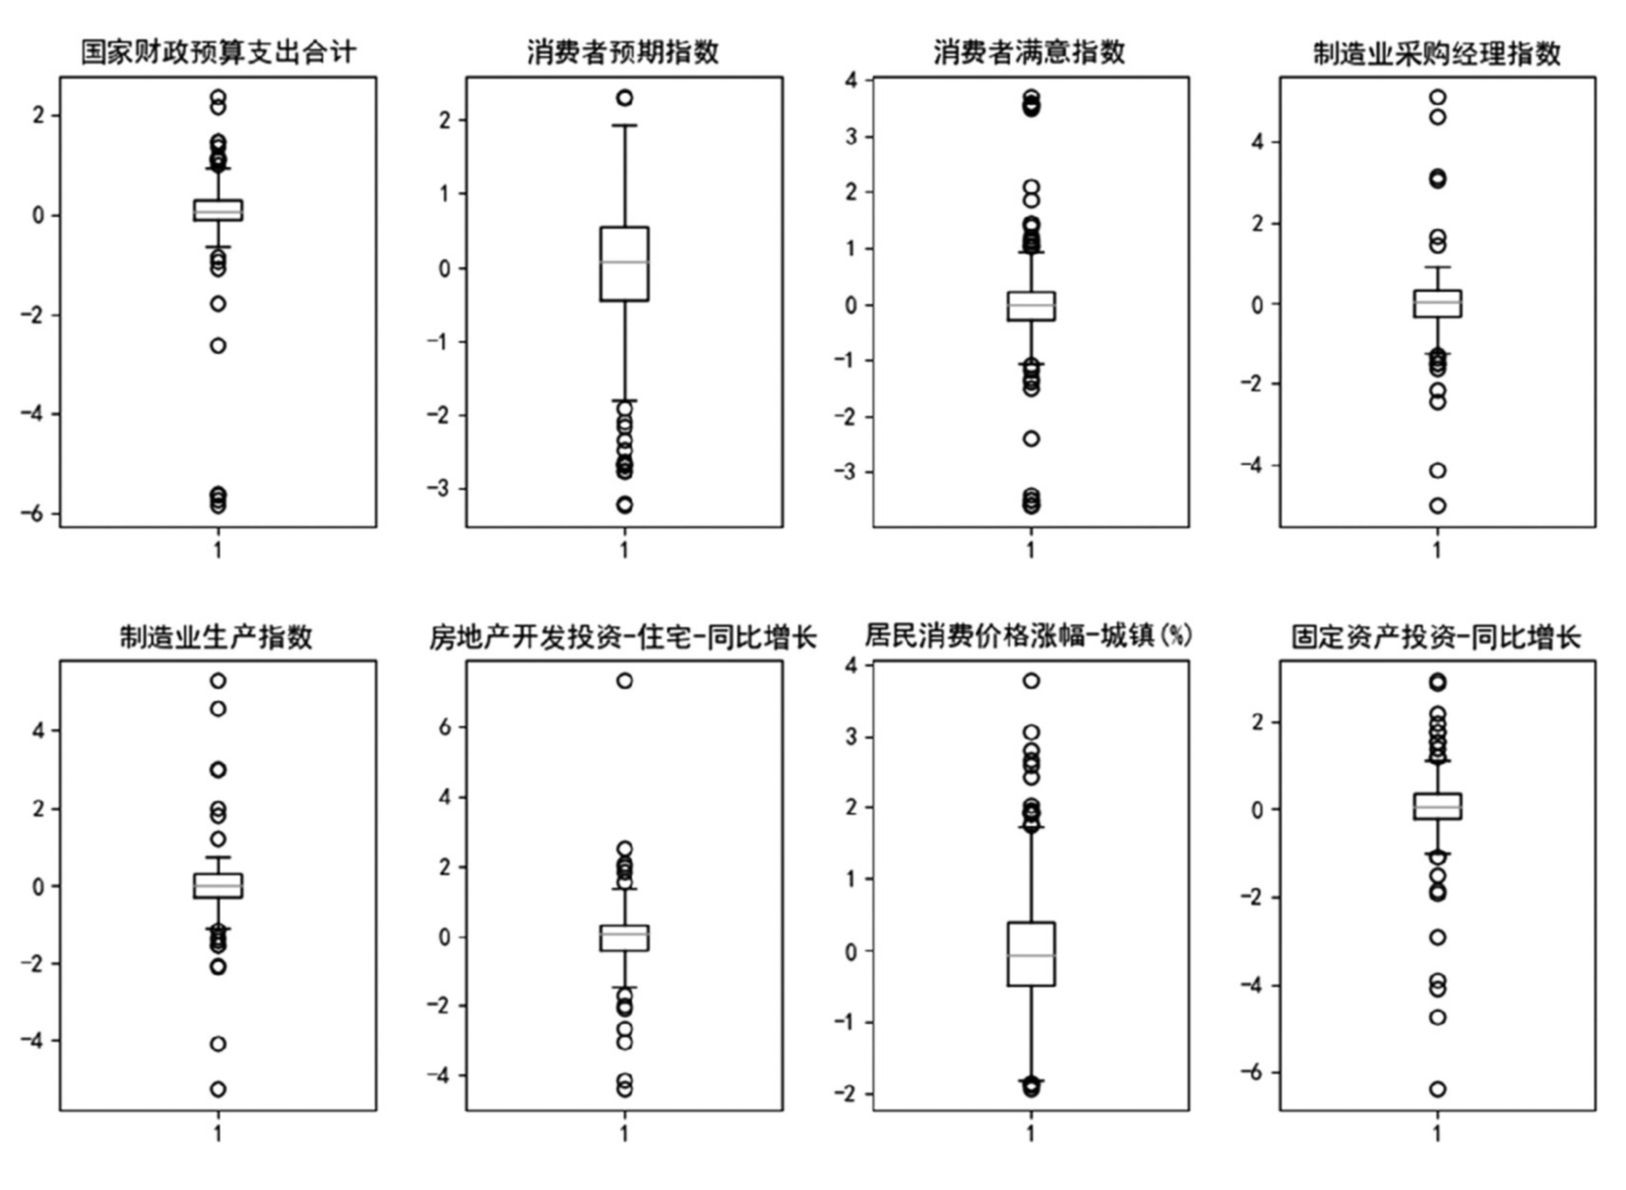
\includegraphics[width=11cm]{pics/some-indexes.jpg}
    \end{minipage}
    \begin{minipage}[t]{1\textwidth}
    \centering
    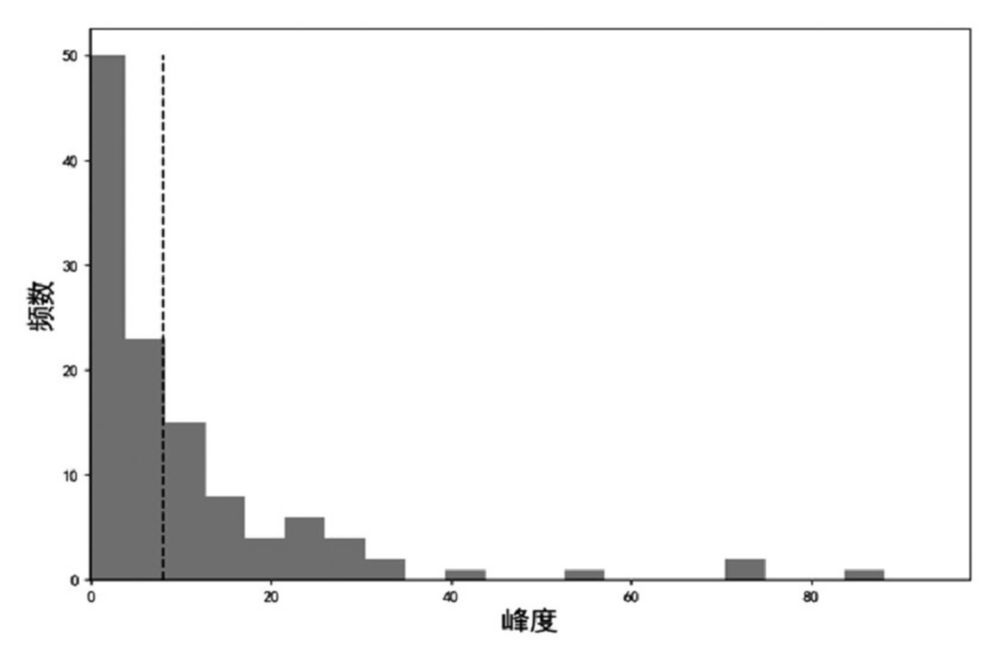
\includegraphics[width=9cm]{pics/fengdu.jpg}
    \end{minipage}
    \caption{\small 部分指标的箱形图和各经济指标的峰度分布情况}
\end{figure}

\subsubsection{实证结果}
参考由Bai与Ng提出的用于选择静态因子个数的信息准则,
我们将由117维月度数据集的共同因子个数定为8个。模型中线性预测模型部分滞后阶数由最小BIC准则给出。
我们分别使用L1方法和PCA估计因子载荷和因子得分,从可以看出,L1方法和PCA得到的因子载荷是有明显区别的。

% Please add the following required packages to your document preamble:
% \usepackage{booktabs}
% \begin{table}[]

%     \begin{tabular}{@{}ccccccccc@{}}
%     \toprule
%       & 因子1       & 因子2              & 因子3        & 因子4      & 因子5          & 因子6         & 因子7           & 因子8           \\ \midrule
%     1 & 先行指数      & 工业增加值增长率         & 海关代征增值税    & 成交金额——股票 & 农村居民消费价格涨幅   & 货币和准货币同比增长  & 游客人数同比增长——亚洲  & 美元价格          \\
%     2 & 货币供应量同比增长 & 工业增加值——私营企业      & 制造业各项税收    & 成交金额——期货 & 城镇居民消费价格涨幅   & 生产经营活动预期指数  & 游客人数同比增长      & 游客人数同比增长——非洲  \\
%     3 & 预警指数      & 工业增加值——股份合作企业    & 财政预算收入     & 成交金额增长率  & 居民消费价格当期     & 存款性公司货币和准货币 & 游客人数同比增长——非洲  & 游客人数同比增长——美洲  \\
%     4 & 制造业采购经理指数 & 工业增加值——国有及国有控股企业 & 关税         & 本月流动股换手率 & 居民消费价格涨幅——居住 & 存款性公司货币同比增长 & 游客人数同比增长——大洋洲 & 工业生产者生产资料价格指数 \\
%     5 & 制造业生产指数   & 工业增加值——重工业       & 房屋新开工面积增长率 & 当月成交金额   & 居民消费价格涨幅——食品 & 住房房屋竣工面积增长率 & 生产经营活动预期指数    & 工业生产者出厂价格指数   \\ \bottomrule
%     \end{tabular}
% \end{table}
\begin{figure}[H]
    \centering
    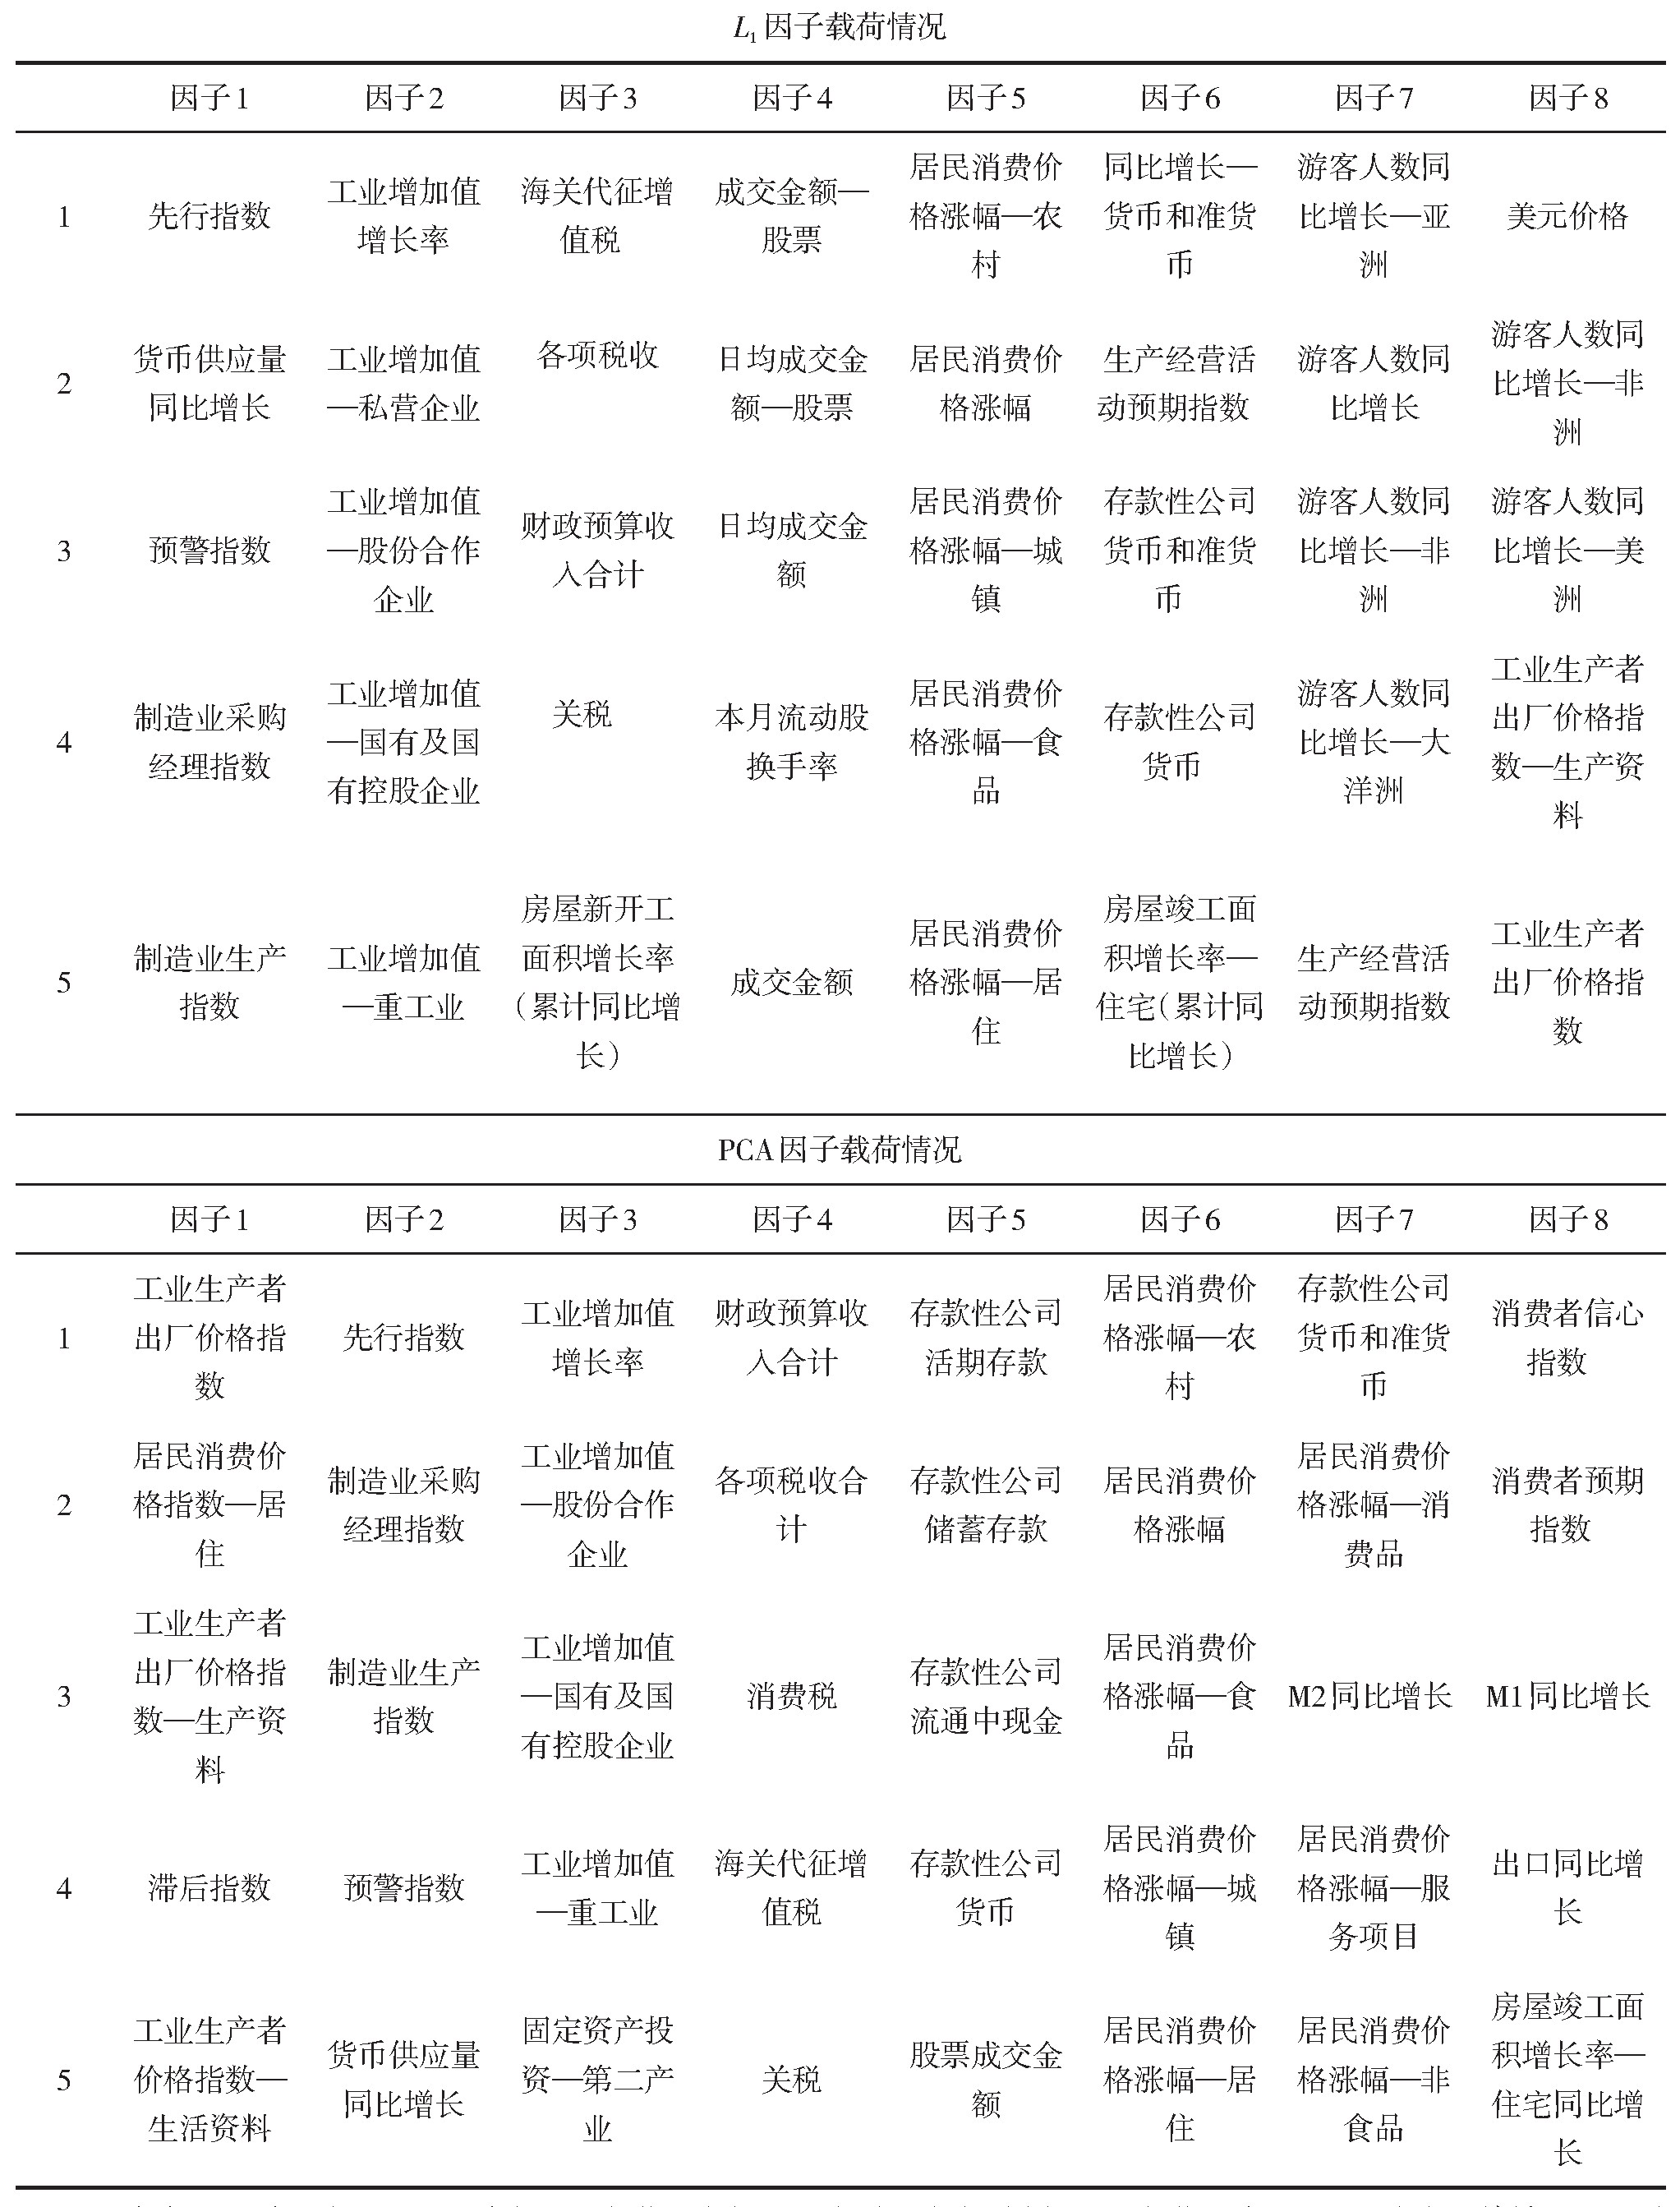
\includegraphics[width=.9\textwidth]{pics/factors.jpg}
    \caption{\small 因子载荷矩阵}
    \label{diff-factors}
\end{figure}

\begin{figure}[H]
    \centering
    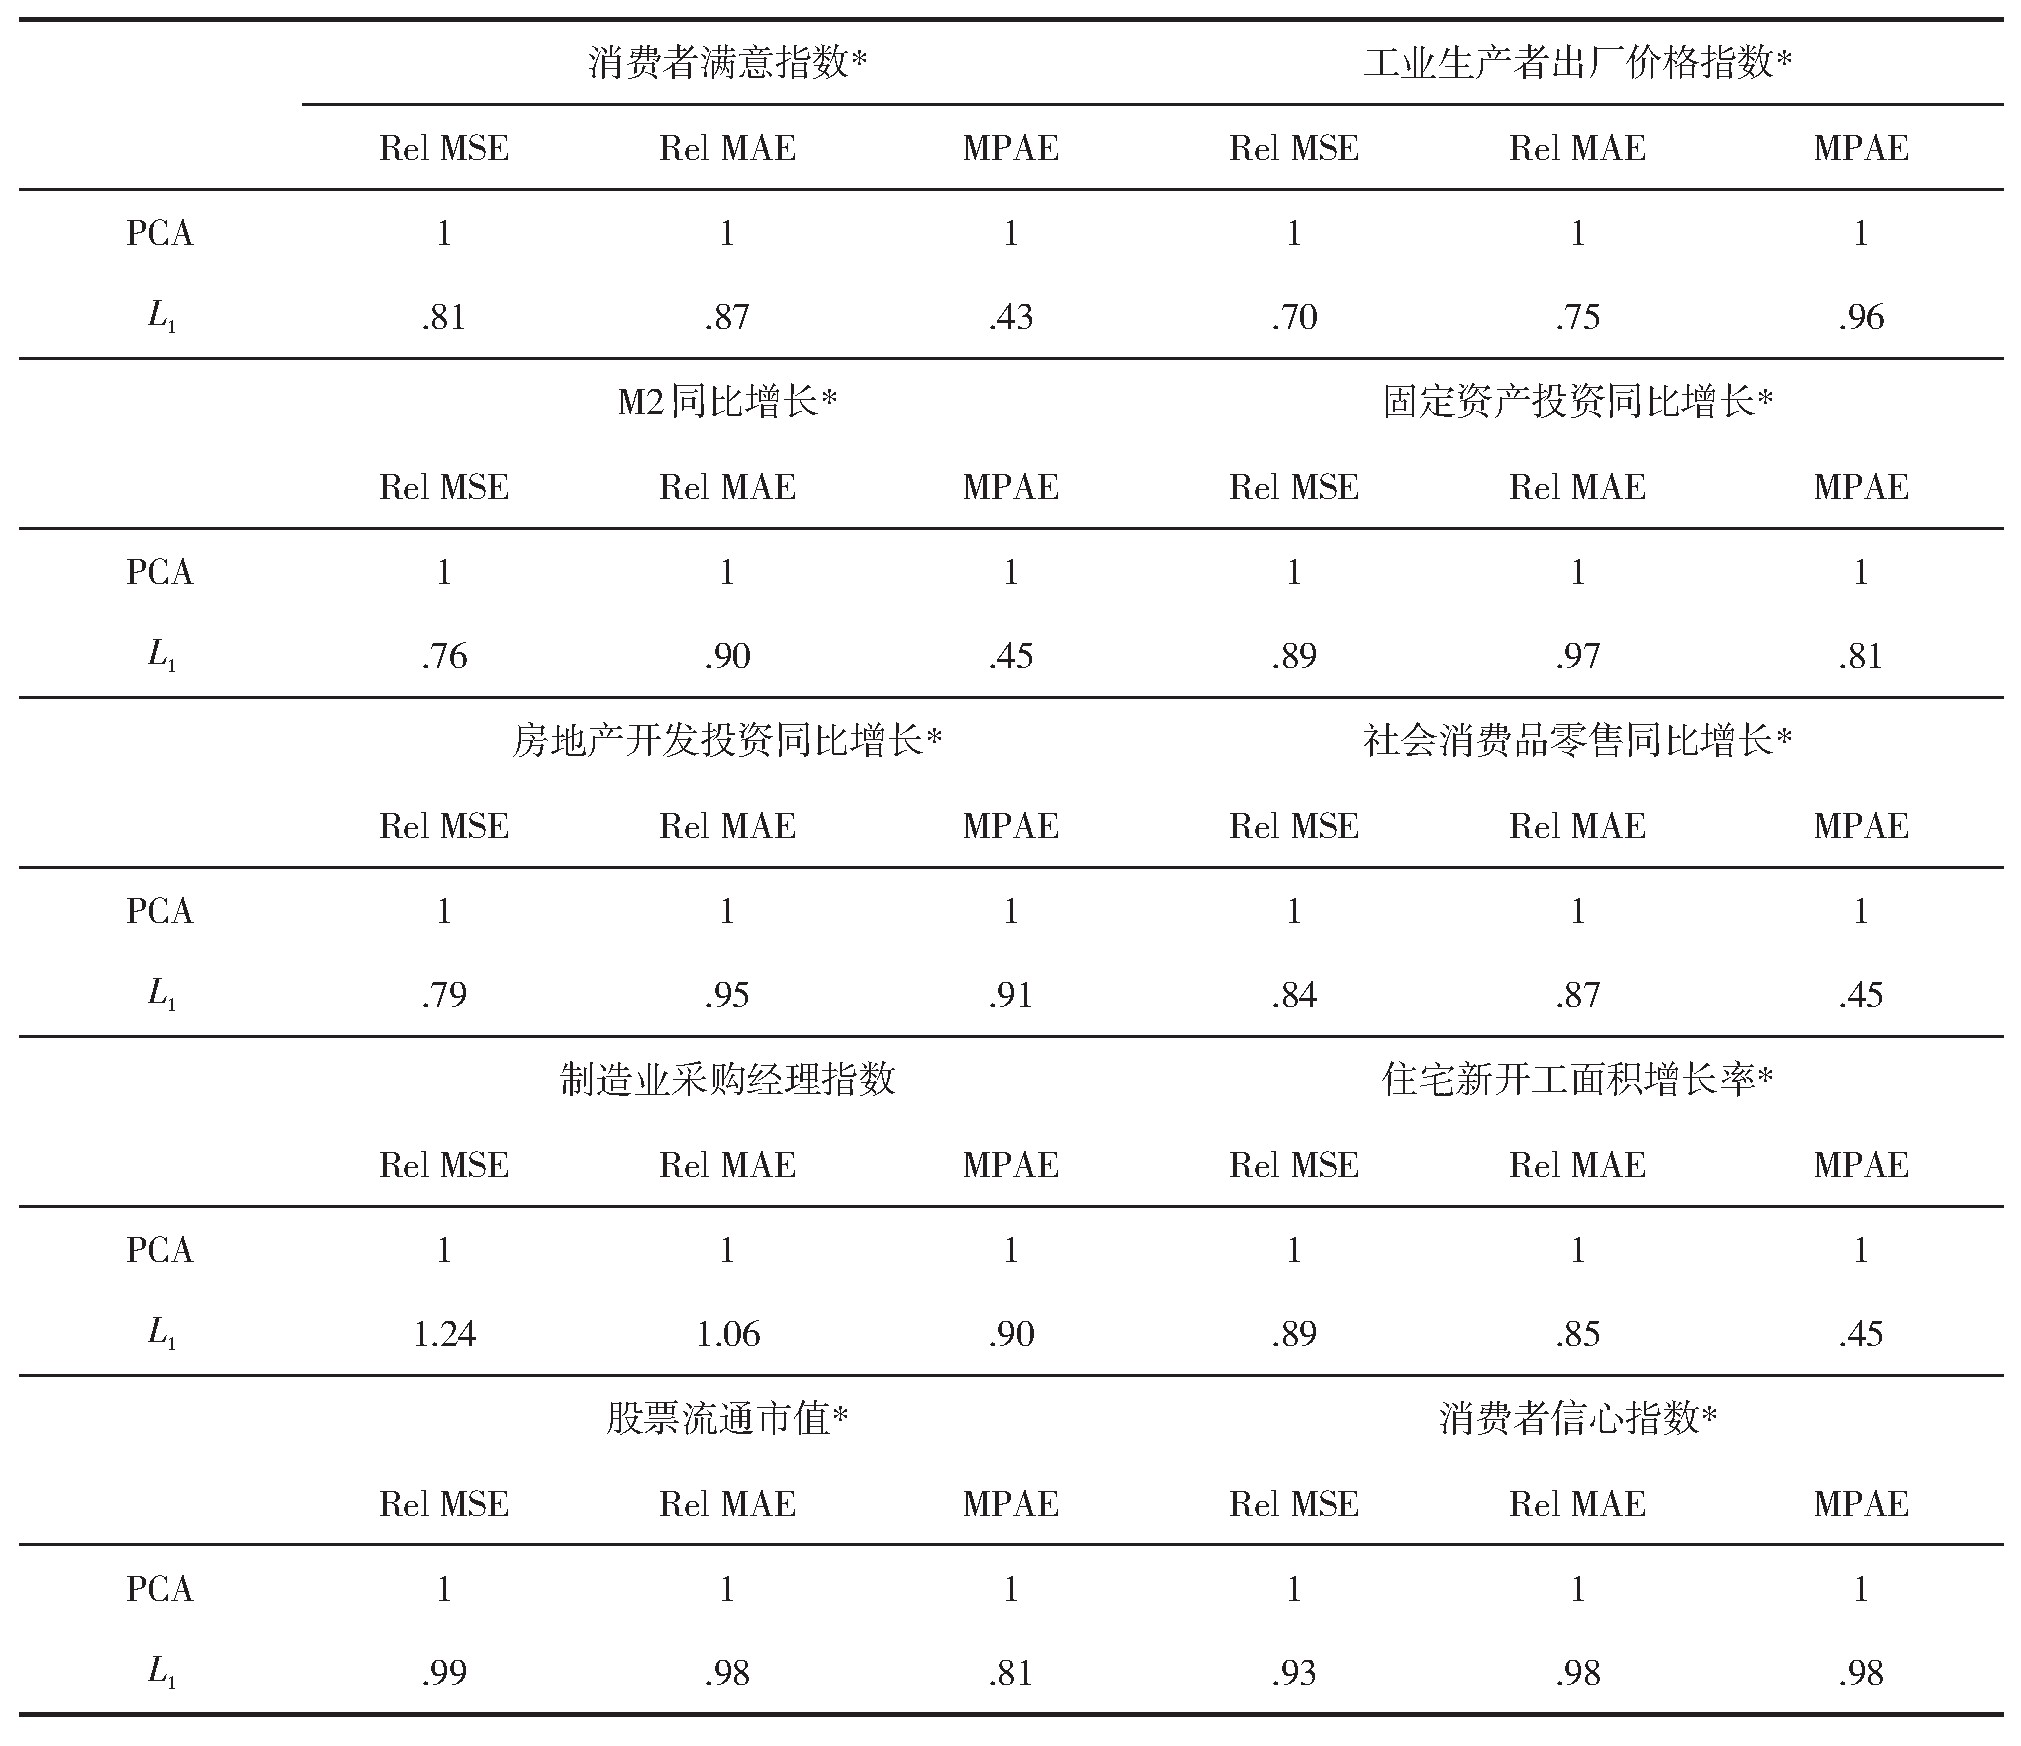
\includegraphics[width=.9\textwidth]{pics/one-month.jpg}
    \caption{\small 向前一个月预测}
    \label{one-month}
\end{figure}


接下来比较PCA估计得出的因子和L1方法得到的因子在指标预测中的表现。
我们在处理后的数据集中选取了10个经济指标,将固定时间长度(180个月)的数据集设为训练数据,
使用滑动窗口预测,并设置预测步长h为1个月、3个月和6个月。并分别比较了两组因子的预测效果,
为比较预测效果选取了三个主要度量标准,即均方误差(MSE)、平均绝对误差(MAE)和平均绝对百分比误差(MPAE)。
每一度量标准均将PCA得到的因子相对值设置为1,见表。


\subsection{本章小结}
本章首先简要介绍了因子模型的基础理论,包括了正交因子模型、动态因子模型和近似因子模型的模型假设和适用场景。
近似因子模型的因子估计量可以用于宏观经济预测,我们着重讨论了它的一种非参数估计——主成分估计量。
主成分分析、奇异值分解等方法都等价于基于$L_2$范数优化问题,都不具有对离群值的稳健性。
针对宏观经济数据往往分布重尾、具有大量缺失和离群值的情况,我们提出了引入$L_1$范数来改善估计的稳健性,并且
提出了基于$L_1$范数的因子模型估计方法。最后,通过模拟实验,验证了基于$L_1$范数的因子模型估计方法的稳健性。